%How it will be Implemented

%\section{Tipps/Notes}
%make plots from the different sensors and the log data to show how it was 
%produced an how it resembles the real data.
The simulation itself is implemented in Matlab as different .m files.

\section{Sensor Model}
How the concept of the different sensor models work is described in chapter \ref{ch:Approach}.
Following here, the implementation which is used in the simulation will be stated in detail.
First in general for all sensors, following by the different characteristics of each sensor.

\subsection{Perfect Sensor}
In general, the perfect sensor data are calculated like stated in chapter \ref{ch:Approach}.

\begin{figure}
 \centering
 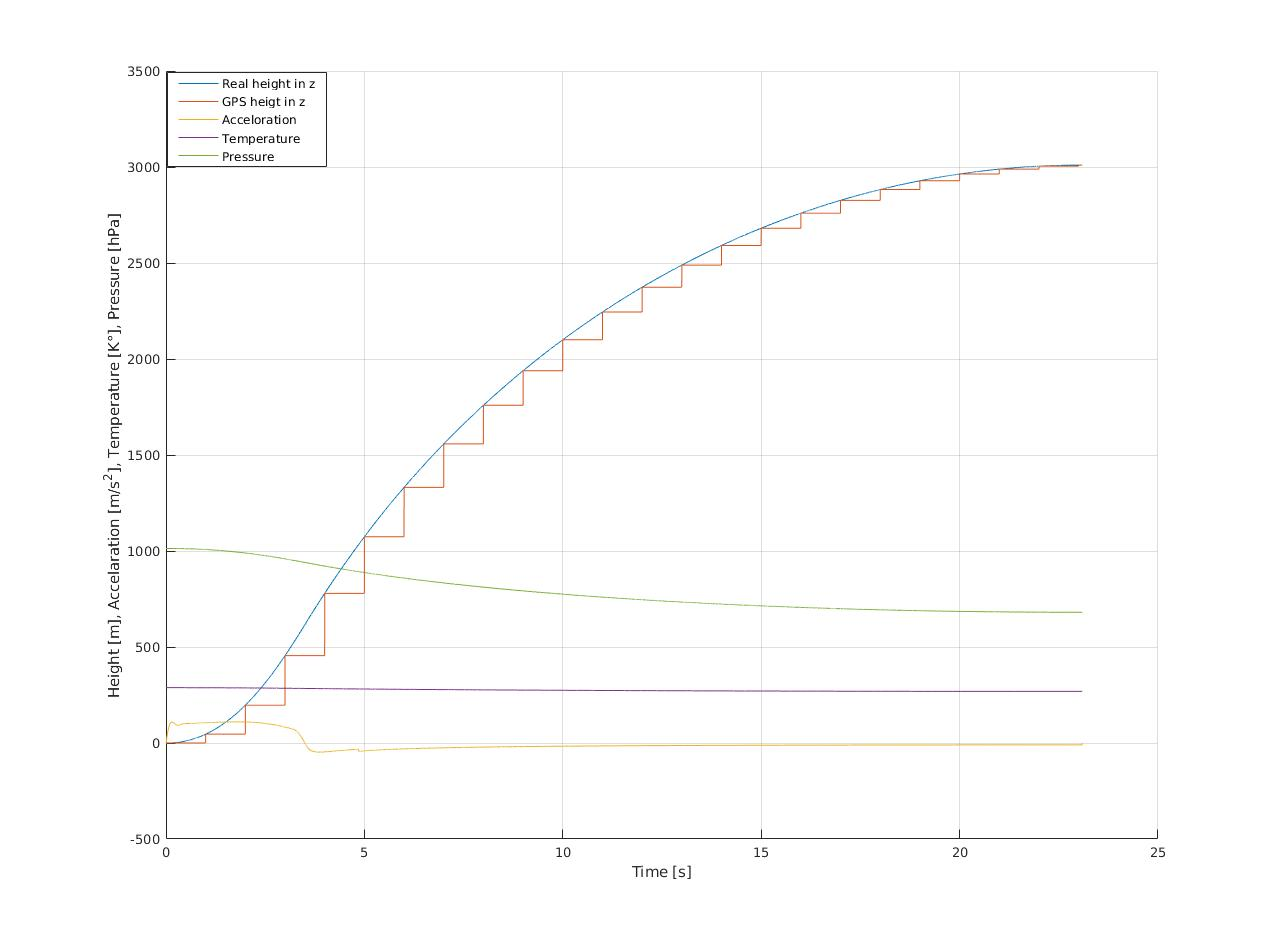
\includegraphics[width=\textwidth]{./Pictures/GeneratedSensorData.jpg}
 % GeneratedSensorData.jpg: 0x0 pixel, 300dpi, 0.00x0.00 cm, bb=
 \caption{Generated sensor data}
 \label{fig:GeneratedPerfectSensor}
\end{figure}

\subsection{Accelorometer}
Due to the fact that whole simulation works with discreet time stamps, the derivative of the height can not be done formally.
So it is done by calculating the difference in each data point to the next and then weight those by the delta in time between them.
This has to be done two times to get from the height to the acceloration.

\subsection{Gyrometer}
The gyrometer measurements are difficult, because it can not be directly calculated from the height.
Therefore the best option to generate this data, is to fit a polynom onto the measured data for the test flights.
I think i should do this tomorrow.

\subsection{Barometer}
\subsubsection{Pressure}
As stated before, the pressure is generated from the height with the help of the international atmospheric model.
\subsubsection{temperature}

\subsection{GPS}
As stated in chapter \ref{ch:Approach} the GPS signal is just the height with a different sampling time. 
To maintain the vectors length which simplifies the later use in the estimation algortihm,
the signal is acquired with a zero order hold convertion instand of a down sampling. 

% Add code for the zero order Holde convertion

\subsection{Noise}
To generate the noise out of the data from the test flight, this has first to be extracted.
It is assumed that the noise on the data is different depending on the state of the rocket (before Icognition, during motor burning, after burnout till parachute ejection),
but it should have more or less the same properties between those events.
Depending on this, the data vector have first to be separated in those different sections.
For this the accelorometer measurements are iterated to find the time stamps on which those events happen like in figure bla.

%% picture of acceloration of z axis with icognition, burnout and parachute ejection are marked

If done so, polynoms are fitted on this measurements with the least squared error method.
Those polynoms represent the function which is assumed to be the noiseless data with possible offsets.
So if now the test flight data is subtracted by those polynomial curves which results in the noise without a mean.
From this point on this noise can be examined on its parameters, like the power density, the probability distribution and the variance figure bla.

%% pictue of autocorrelation, histogramm etc from sensor data noise

This noise data can now used tho solve the yule walker equation to get an AR-model.
But first, the data has to be resampled so that the AR-models can be used proper in the simulation.
With those AR-models, the noise can be regenerated by filtering white noise with the correct variance.
This generated noise can now be compared to the noise form the test flight data.

%% picture of pwelch plot from both noise vectors

As seen in figure bla those noise resemble each other in their power density spectrum much more the white noise would.
So the AR-model is exported to the simulation script an can there be used to generated the real sensor data.

\subsection{Accelorometer}
The noise which is on the accelorometer is special because it often has a drift which results in a more or less constant offset.
To recreate this, the offset can be estimated from the test flight data.
Especially the data before the icognition are help full, because the value that should be measured is known.

\subsection{Gyrometer}


\subsection{GPS}
The noise capacites of GPS is not real white. It more resembles a brown noise because it has a slow ocsillation over it.
I have to determine how i will remodel this in perticular.

\subsection{Real Sensor}
To now generated the real sensor data, the different noises have to be generated like stated above.
For this a vector of normal distributed random values is generated and multiplied by the square root of the corresponding variance.
This white noise is now filtered by the corresponding AR-model and can then be added onto the corresponding perfect sensor data.
This now results in the real sensor data.

\subsection{Accelorometer}
To generate the real sensor data of the 

\subsection{Gyrometer}

\subsection{Barometer}

\subsection{GPS}





\section{System Model}
6*6 with moving point mass and temperature.
4*4 with just temperature.
3*3 just moving point mass.

\section{State Estimator}
\subsection{}
\subsection{Loop}
